\documentclass[runningheads]{llncs}

\usepackage{tikz}

\usepackage{amsmath,amssymb}
%\usepackage{amsthm}
%\usepackage{unicode-math}
\usepackage{tikz}
\usetikzlibrary{external}
\usepackage{hyperref}
\usepackage{nccrules}
\AtBeginDocument{\renewcommand\setminus{\smallsetminus}}


\newcommand\mpar[1]{{\left(#1\right)}}
\newcommand\mbrk[1]{{\left[#1\right]}}
\newcommand\mbrc[1]{{\left\{#1\right\}}}
\newcommand\mdbrk[1]{\left?#1\right?}
\newcommand\card[1]{{\left|#1\right|}}
\newcommand\psubst[1]{\mbrc{\!\!\mbrc{#1}\!\!}}
\newcommand\subst[2]{\mbrk{#1\middle/#2}}
\newcommand\midbar{\,\middle|\,}
\newcommand\mset[2]{\mbrc{#1\midbar #2}}

\newcommand\act{\mathrm}
\newcommand\OA[6]{\left<#1,#2,#3,#4,#5,#6\right>}
\newcommand\OTbase[4]{\text{\small\(%
	\setlength\arraycolsep{2pt}\everymath{\displaystyle}%
	\renewcommand\arraystretch{1}%
	\begin{array}{c}%
	#2,#3,#4 \\\noalign{\color{red}\hrule\vspace{1pt}\hrule}
	#1
	\end{array}\)}}
\newcommand\OThelperdonotuse[2][\top]{\OTtemporary{#1}{\mbrc{#2}}}
\newcommand\OTd[2]{\newcommand\OTtemporary{\OTbase{#1}{\mbrc{#2}}}\OThelperdonotuse}
\newcommand\OT[3]{\OTbase{#1\xrightarrow{\raisebox{-1.5pt}[.8\height][0pt]{\makebox[1.4\width]{\(\scriptstyle #3\)}}}#2}}
\newcommand\OTx[4]{\OT{s_{#1}}{s'_{#1 #2}}{\alpha_{#1 #2}}{\beta_{#3 j}^{j \in J'_{#4}}}{g_{#1 #2}}{\psi_{#1 #2}}}
\newcommand\OTg{\OTx{}{}{}{}}
\theoremstyle{plain}
\newtheorem{thm}{Theorem}
\newtheorem{lem}{Lemma}
\newtheorem{cor}{Corollary}
\newtheorem{prop}{Proposition}

\theoremstyle{definition}
\newtheorem{defi}{Definition}
\newtheorem{exi}{Example}

\newcommand\comment[3]{\colorbox{#1}{#2}\marginpar{#3}}
\newcommand\Rabea{\comment{yellow}}
\newcommand\Ludo{\comment{green}}
\newcommand\Eric{\comment{cyan}}
\newcommand\Quentin{\comment{pink}}

\newcommand\nmm[1]{\(\displaystyle #1\)} % nmm for Nice Math Mode
\newcommand\hyp[1]{\TextOrMath{(H\textsubscript{#1})}{\tag{H\textsubscript{#1}}}}
\newcommand\goal[1]{\TextOrMath{(#1)}{\tag{#1}}}
\newcommand\defitem{\item[\bullet]}

\newcommand\setR{\mathbb{R}}
\newcommand\setZ{\mathbb{Z}}
\newcommand\setN{\mathbb{N}}

\newcommand\choice[1]{\left\{\everymath{\displaystyle}%
	\begin{array}{lr}#1\end{array}\right.}
\newcommand\subbox[1]{{\makebox[.5\width]{\(\scriptstyle #1\)}}}
\newcommand\bigsymb[2][\Large]{\text{#1\nmm{#2}}} % DeclareMathDelimiter?
\newcommand\defnotation{\DOTSB\;{\Colon=}\;}
\newcommand\defobject{\DOTSB\;{\coloneq}\;}
\newcommand\nwedge{\DOTSB\;{\wedge}\;} % when you want to force space
\newcommand\qwedge{\DOTSB\quad{\wedge}\quad}
\newcommand\wrel[4][]{{#2 \overset{#1}\leq_{#4} #3}}
\newcommand\fvars[1]{{\mathit{vars}\mpar{#1}}}
\newcommand\fguard[1]{{\mathit{guard}\mpar{#1}}}
\newcommand\fOT[1]{{\mathrm{OT}\mpar{#1}}}
\newcommand\terms{{\mathcal{T}}}
\newcommand\rterms[1]{{\mathcal{T}_{\!\! #1}}}
\newcommand\cterms{\rterms{\emptyset}}
\newcommand\formulae{{\mathcal{F}}}
\newcommand\rformulae[1]{{\mathcal{F}_{\!\! #1}}}
\newcommand\cformulae{\rformulae{\emptyset}}
\newcommand\values{{\mathcal{P}}}
\newcommand\actions{{\mathcal{A}}}
\newcommand\reach[1]{{\checkmark_{\!\! #1}}}
\tikzstyle{every edge} = [draw,-latex,every node/.style={auto}]
\tikzstyle{state} = [draw,circle,minimum size=1cm,inner sep=1mm]
\tikzstyle{initial} = [double,double distance=1mm,minimum size=.95cm,inner sep=.5mm,outer sep=.5mm]
\tikzstyle{init} = [double,double distance=1.5pt,edge label=\(\mbrc{#1}\)]
\tikzstyle{dir} = [out=#1+15,in=#1-15,looseness=10]


\begin{document}
%
\title{Refinements for open pNets}
%
%\titlerunning{Abbreviated paper title}
% If the paper title is too long for the running head, you can set
% an abbreviated paper title here
%
\author{
Rabéa\inst{1}\orcidID{1111-2222-3333-4444} \and
Quentin\inst{1,2}\orcidID{1111-2222-3333-4444} \and
Ludo\inst{2}\orcidID{0000-1111-2222-3333} \and
Eric\inst{3}\orcidID{2222--3333-4444-5555}}
%
\authorrunning{Rabéa Ameur-Boulifa et al.}
% First names are abbreviated in the running head.
% If there are more than two authors, 'et al.' is used.
%
\institute{blabla
\email{lncs@fff}\\
\url{http://www.springer.com/gp/computer-science/lncs} \and
blibli\\
\email{\{abc,def\}@fff}}
%
\maketitle              % typeset the header of the contribution
%
\begin{abstract}
 The abstract should briefly summarize the contents of the paper in
150--250 words.

Establishing equivalences and refinement relations between programs is an important mean for 
verifying the correctness of programs, by formally proving the relation between a specification and an implementation, 
proving that two implementation are equivalent, or justifying optimisations and transformations, by establishing that the
behaviors of a modified program simulate those of to the source one.

In this article, we discuss a notion of refinement between so-called "open automata", which are symbolic
behavioral models for communicating systems. Open automata may have "holes" modeling elements of their
context, and can be composed by instanciation of the holes. This allows for a compositional approach for
verification of their behavior, essential to address proofs about large realistic systems.

We define several variants of refinement between systems including either equal or different sets of holes, and 
show under which conditions these refinements are preserved by composition of open automata. We also discuss
the relations between these refinements and the existence of deadlocks.
We illustrate these notions on several simple use-cases.


\keywords{Labelled transition systems  \and Refinement \and Composition.}
\end{abstract}
%
%
%
\section{Introduction}
\TODO{1.5 pages}


\section{Related Work}
\label{sec:sota}

\TODO{1 page}

Previous work on open automata focused on equivalence relations compatible with composition.
In an article by Hou, Zechen and Madelaine \cite{10.1145/3372884.3373161}, a computable bisimulation is introduced and proved equivalent to the previous bisimulation already introduced.
In a more recent work by Ameur-Boulifa, Henrio and Madelaine \cite{2007.10770}, a weak version of the bisimulation on open automata is introduced.
These works differ from ours because the relation introduced in this report is a refinement relation in the form of a simulation and not a bisimulation.
Also we do not have results as strong as computability neither a weak version able to tackle silent actions.

Some related work on other models than open automata introduce refinement relations.
In a chapter by Bellegarde, Julliand and Kouchnarenko \cite{10.1007/3-540-46428-X_19}, a simulation relation on transition systems is introduced.
This simulation encompass action refinement, is able to deal with silent actions and is compatible with parallel composition.
Here the refinement relation does not consider action refinement as valid but it should be done in future work.
Also they check how LTL properties are preserved or combined using their refinement which we do not do.
However their model is less expressive: the transition system model is less expressive than open automata and the parallel composition is less expressive than composition on open automata.
In a later report by Kouchnarenko and Lanoix \cite{10.1007/978-3-540-70881-0_26}, the refinement relation they introduce is on LTS (labelled transition systems).
Their relation additionally prevents deadlock and livelocks.
The composition is also extended to synchronised composition which is more expressive.
In our work we also deal with deadlocks but not with livelocks since the latter arise only with silent actions.
This work is closer than the previous one to what we do here, still open automata are more expressive than LTS and composition is more general than sychronised composition.

A refinement relation on models nearer to open automata is introduced in an article by Zhang, Meng and Lo \cite{Zhang2014}.
In their article they work with transition systems with variable which makes the state space potentially infinite.
This aspect is also present in open automata.
They show how invariants, a notion near to our reachability predicates, are composed.
By relation on these invariants they introduce several refinement relations.
We could have done something similar for non-locking composition reachability predicates which are introduced in Section \ref{sec:proofelts}.

On the deadlock prevention aspect, an article by Dihego, Sampaio and Oliveira \cite{DIHEGO2020110598} present a refinement relation on process algebra (translated to LTS).
This refinement relation is a special case of inheritance and prevents the introduction of deadlocks.
Their refinement and inheritance are quite the opposite of our refinement in terms of new behaviours.
They have channels, interfaces, inputs and outputs, which in the open automata model can be compared to action labels, holes and action data for both inputs and outputs.
They have a rich composition as open automata but the introduction of deadlock is already prevented by a well chosen set of composing operations.
Also their composition is slightly different than the one on open automata because they can cause loops by linking two channels of the same process, where in open automata the composition makes an oriented tree.
In their model there is an explicit deadlock and a succesful termination where in open automata there are no explicit termination.
We define a deadlock as a configuration without possible transition and assume what is a deadlock when comparing the open automata.
To define their refinement and inheritance relation they use trace and failure semantics, which are weaker than (bi)simulations \cite{10.5555/640428.640430} and could break with open automata compositon.


\section{Background: Open Automata and their Composition}\label{sec:background}
\TODO{3.5 pages}

This section presents the notations we used and the principles of automata. Except for minor changes in the notations, the only new contribution of this section is the definition of a composition operator for open automata.
%
%Notations will be defined with the operator \(\defnotation\) and names are given with the operator \(\defobject\) as follows:
%\begin{align*}
%	\mathit{notation\_with\_variables} & \defnotation \mathit{notated\_object\_using\_the\_variables} \\
%	\mathit{name} & \defobject \mathit{fully\_defined\_mathematical\_object}
%\end{align*}

%Throughout this paper, tuples will be noted differently depending on what they represent.
%This helps distinguishing the manipulated objects.
%Every such notation will be introduced in the definition of the object.

Families of values, or equivalently maps will be noted \(\mset{i \mapsto x_i}{i \in I}\), \(\mset{i \gets x_i}{i \in I}\) or \(x_i^{i \in I}\). % TODO: introduire le fait que \exists c_j^{j \in J} défini J et {j \mapsto c_j}
%For instance \(\mpar{ax}^{x \in \setR}\) represents a scaling function, \(c^{i \in I}\) is a constant function over \(I\).
%They will be used depending on what is more convenient.
%For instance \(\mbrc{\alpha \mapsto 1, \beta \mapsto 2, \gamma \mapsto 3}\) has no simple generating expression and is better represented with the finite version of first notation.
The disjoint union on set is noted \(\uplus\)\footnote{\(\uplus\) notation either supposes that the sets are disjoint or rename conflicting objects depending on the context}. Disjoint union is also used on maps.
%There are several ways of ensuring a union is disjoint, we will indifferently either suppose sets are disjoint or rename conflicting object (useful for variables).
%The disjoint union of two maps \(\varphi: I \to X\) and \(\psi: J \to Y\) with \(I \cap J = \emptyset\) is noted \(\varphi \uplus \psi\) and has the following signature \(I \uplus J \to X \cup Y\).
In a formula, a quantifier followed by a finite set will be used as a shorthand for the quantification on every variable in the set:
\(\forall \mbrc{a_1, \dots, a_n}, \exists \mbrc{b_1, \dots, b_m}, P\) means \(\forall a_1, \dots, \forall a_n, \exists b_1, \dots, \exists b_m, P\).

%\begin{definition}[Expression algebra, Action algebra, Formulas, Terms]
An expression algebra \(E\) is the disjoint union  of  terms,  actions, and  formulas
\( E=\terms \uplus \actions \uplus \formulas\) .
\(\terms\) and \(\actions\) are term algebras.
The formulas \(\formulas\) contain at least first order formulas and equality\footnote{Equality does not need to be only syntactic.} over \(\terms\) and \(\actions\).
%\end{definition}

 \(\fvars{e}\) is the set of variables in \(e \in E\) that are not bound by any binder. An expression is closed if \(\fvars{e}=\emptyset\).
The set \(\values\) denote values which is a subset of closed terms.

The substitution in \(e \in E\) of \(x \in \fvars{e}\) by \(t \in \terms\), is denoted \(e\subst{t}{x}\), and its generalisation to the parallel substitution of variables in \(V\) by \(\psi: V \to \terms\) is denoted \(e\psubst{\psi}\).


 We suppose given a decidable satisfiability relation on formulas, \({\vdash} f\) is the satisfiability over closed formulas.
% In practice one of our objective is to be able to use a SMT solver to reason automatically on the properties of open automata, in this case
%\(\vdash\) can hence be interpreted as an indicator of what is given to the SMT; it separates the external logic and the logic on \(\formulas\).
We will  use two satisfiability relations:
\begin{itemize}
\item The satisfiability of a formula \(f \in \formulas\) under some valuation \(\sigma: V \to \values\):
\( \sigma \vdash f ::= \vdash \exists \fvars{f\psubst{\sigma}}, f\psubst{\sigma} \)
\item The satisfiability of a formula \(f \in \formulas\) with some variable set \(V\) as context:
\( V \vdash f ::=  \vdash \forall V, \exists\mpar{\fvars{f} \setminus V}, f \)
\end{itemize}

%For instance a formula with quantifiers on variables might not be provable even if it is true for all values of these variables.

\subsection{Open Automata}\label{sec:def}
 Open automata are labelled transition systems with variables  that can be used to compose other automata: they are made of transitions that are dependent of the actions of ``holes'', a composition operation consists in filling a hole with another automaton to obtain a more complete automaton. The variables makes the automata symbolic, and the holes allow for a partial definition of the behaviour.

\begin{definition}[Open transition, Open automaton]
An \emph{open automaton} is a tuple \(\OAg\) with \(S\) the set of states, \(s_0 \in S\) the initial state, \(V\) the finite set of variable names, \(\sigma_0: V' \to \values\) the initial valuation of variables where \(V' \subseteq V\), \(J\) the set of hole names and \(T\) the set of open transitions.

An \emph{open transition} is a tuple \nmm{\OTg} with \(s, s' \in S\) the source and target states, \(\alpha \in \actions\) the produced action, \(J' \subseteq J\) the holes involved in the transition, \(\beta_j \in \actions\) the actions of the holes, \(g \in \formulas\) the guard and \(\psi: V \to \terms\) the variable assignments.
\end{definition}

The following terminology will be used to reason on open automata
\begin{definition}[Configuration, instantiated transition]
A pair of a state and a valuation is called a \emph{configuration}.
An \emph{instantiated transition} of an automaton \(\OAg\) is a transition  \(t\psi\) where $t\in T$ and $\psi$ is a  well-formed substitution of the unbound variables of $t$  minus the automaton variables $V$.
\end{definition}

\paragraph{Open automaton composition}

TODO

\paragraph{A bisimulation for open automata}

TODO

\subsection{Example}

As an example, the traffic light system  that controls  
 traffic at the intersection of a busy highway. The open automaton  
modeling this system  is illustrated in  Figure \ref{fig:tls}. This automaton has three states  remembering which coloured light
is on (Red, Yellow or Green). It includes two holes: a controller ($\symb{ctl}$) and a counter ($\symb{cnt}$)  depicting together the behaviour of the timer. The color switches when the counter and the controller component agree that the time is over. The new time limit can be set by the counter component and the exposed action to the environment is an unobservable  action $\tau$.

The open automata shown in Figure  \ref{fig:ctlandcnt} models  the timer. On the left, the controller component designed to be connected in the hole $\symb{ctl}$.  Its role is to decide the duration before switching the lights. 
We control the time interval for each light by setting them by prior knowledge:  17s for the first duration, 3s for the second, and 20s for the third. On the right, the tick counter component designed to be connected in the hole $\symb{cnt}$. It measures elapsed model time in ticks by counting ticks until the time limit retrieved beforehand is reached, then emits an over action with the elapsed time and restart.

In Figure \ref{fig:tlf} we present the composition of the three automata. Each state of the result of the composition consists  of  a state of traffic light system together with a state of controller component and one of counter component.  



\begin{figure}
\centering
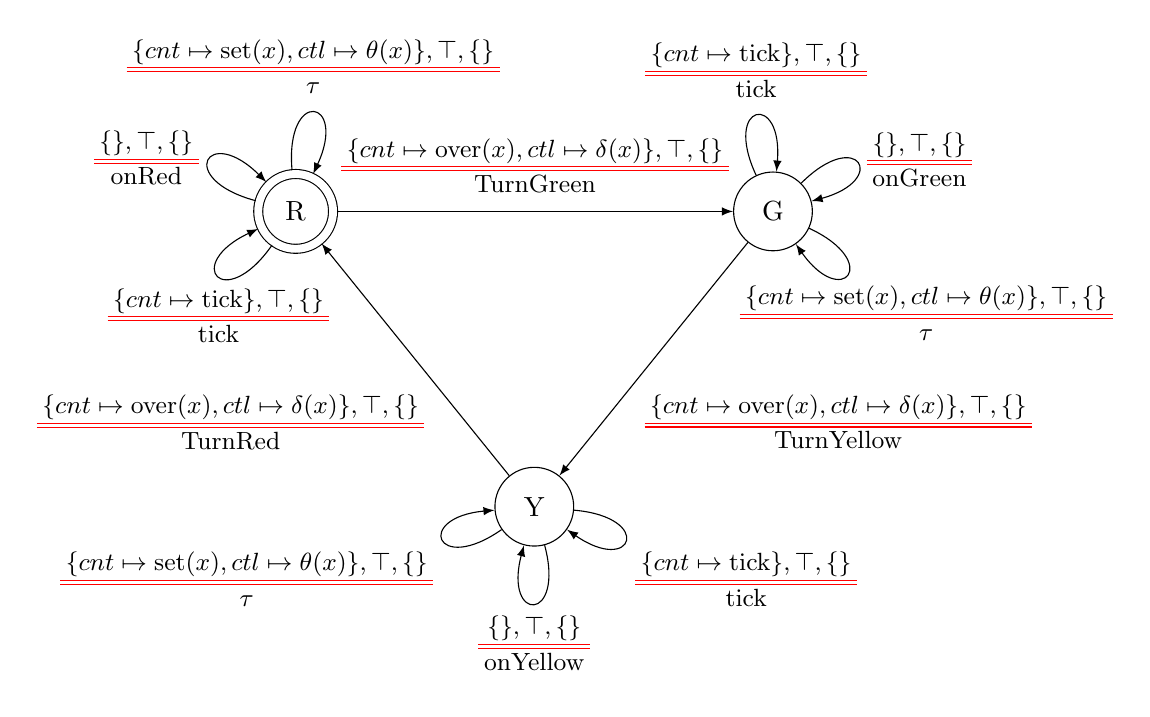
\begin{tikzpicture}

\node[state,initial] (v1) at (150:3.5) {R};
\node[state] (v2) at (30:3.5) {G};
\node[state] (v3) at (270:2) {Y};

\draw (v1) edge[dir=220] node[below] {\OTd{\act{tick}}{cnt \mapsto \act{tick}}{}} (v1);
\draw (v1) edge[dir=150] node[left] {\OTd{\act{onRed}}{}{}} (v1);
\draw (v1) edge[dir=80] node[above] {\OTd{\tau}{cnt \mapsto \act{set}\mpar{x}, ctl \mapsto \theta\mpar{x}}{}} (v1);
\draw (v1) edge node {\OTd{\act{TurnGreen}}{cnt \mapsto \act{over}\mpar{x}, ctl \mapsto \delta\mpar{x}}{}} (v2);
\draw (v2) edge[dir=100] node[above] {\OTd{\act{tick}}{cnt \mapsto \act{tick}}{}} (v2);
\draw (v2) edge[dir=30] node[right] {\OTd{\act{onGreen}}{}{}} (v2);
\draw (v2) edge[dir=320] node[xshift=1cm,below] {\OTd{\tau}{cnt \mapsto \act{set}\mpar{x}, ctl \mapsto \theta\mpar{x}}{}} (v2);
\draw (v2) edge node[pos=0.6] {\OTd{\act{TurnYellow}}{cnt \mapsto \act{over}\mpar{x}, ctl \mapsto \delta\mpar{x}}{}} (v3);
\draw (v3) edge[dir=340] node {\OTd{\act{tick}}{cnt \mapsto \act{tick}}{}} (v3);
\draw (v3) edge[dir=270] node {\OTd{\act{onYellow}}{}{}} (v3);
\draw (v3) edge[dir=200] node {\OTd{\tau}{cnt \mapsto \act{set}\mpar{x}, ctl \mapsto \theta\mpar{x}}{}} (v3);
\draw (v3) edge node[pos=0.4] {\OTd{\act{TurnRed}}{cnt \mapsto \act{over}\mpar{x}, ctl \mapsto \delta\mpar{x}}{}} (v1);

\end{tikzpicture}

\caption{The specification of a Traffic Light system}
\label{fig:tls}
\end{figure}


\begin{figure}
%\centering
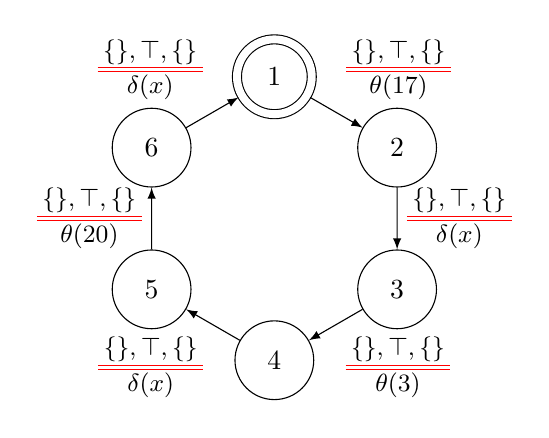
\begin{tikzpicture}[scale=0.60]

\node[state,initial] (v1) at (90:3) {1};
\node[state] (v2) at (30:3) {2};
\node[state] (v3) at (330:3) {3};
\node[state] (v4) at (270:3) {4};
\node[state] (v5) at (210:3) {5};
\node[state] (v6) at (150:3) {6};

\draw (v1) edge node {\OTd{\theta\mpar{17}}{}{}} (v2);
\draw (v2) edge node {\OTd{\delta\mpar{x}}{}{}} (v3);
\draw (v3) edge node {\OTd{\theta\mpar{3}}{}{}} (v4);
\draw (v4) edge node {\OTd{\delta\mpar{x}}{}{}} (v5);
\draw (v5) edge node {\OTd{\theta\mpar{20}}{}{}} (v6);
\draw (v6) edge node {\OTd{\delta\mpar{x}}{}{}} (v1);

\end{tikzpicture}

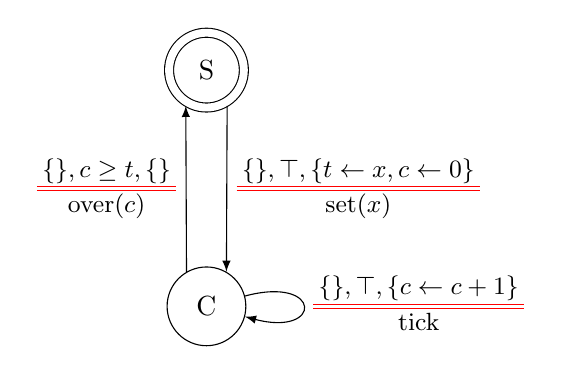
\begin{tikzpicture}

\node[state,initial] (v1) at (0,1.5) {S};
\node[state] (v2) at (0,-1.5) {C};

\draw (v1) edge[bend left,looseness=0] node {\OTd{\act{set}\mpar{x}}{}{t \gets x, c \gets 0}} (v2);
\draw (v2) edge[dir=0] node {\OTd{\act{tick}}{}{c \gets c + 1}} (v2);
\draw (v2) edge[bend left,looseness=0] node {\OTd{\act{over}\mpar{c}}{}[c \geq t]{}} (v1);

\end{tikzpicture}
\caption{(a) An example of controller component ~~  (b) An example of counter component}
\label{fig:ctlandcnt}
\end{figure}



\begin{figure}
\centering
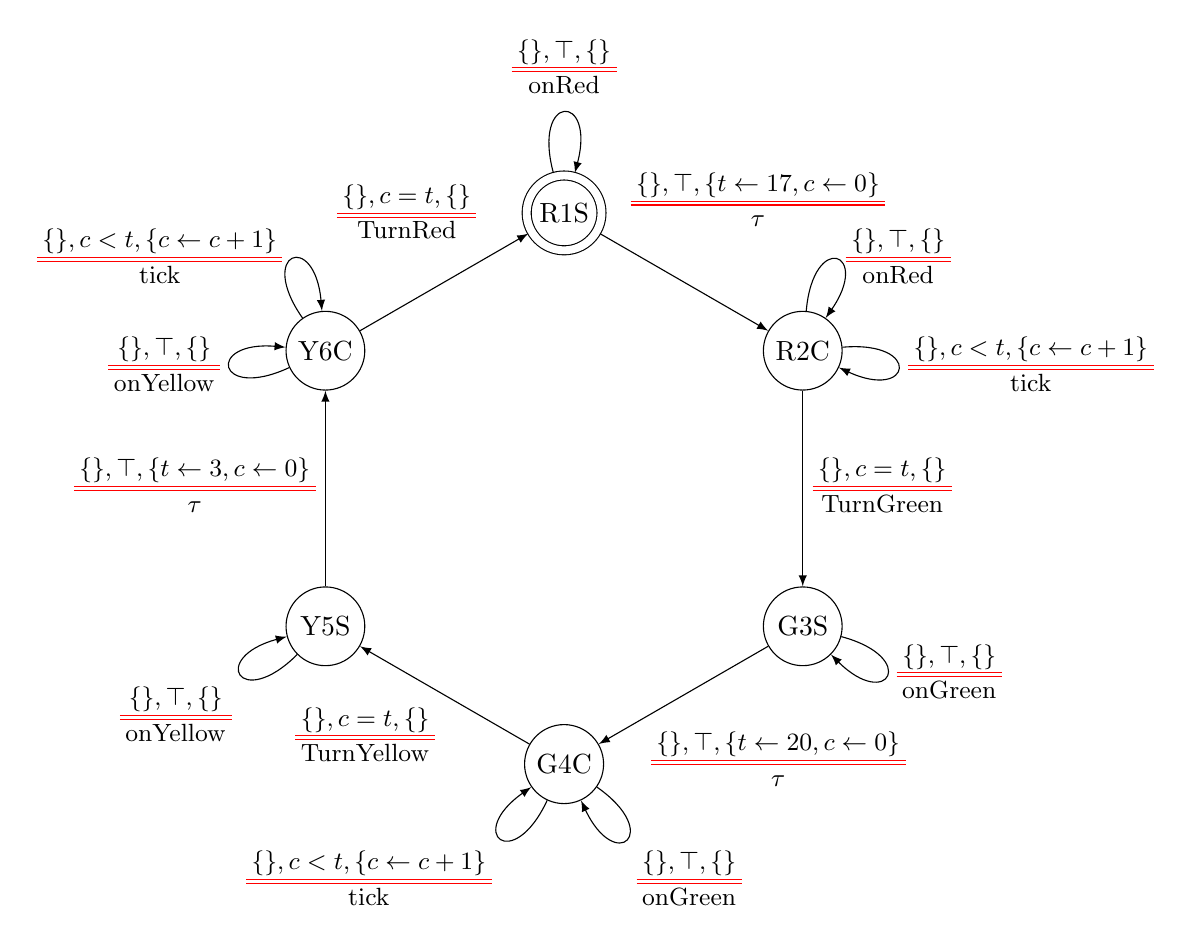
\begin{tikzpicture}

\node[state,initial] (v1) at (90:3.5) {R1S};
\node[state] (v2) at (30:3.5) {R2C};
\node[state] (v3) at (330:3.5) {G3S};
\node[state] (v4) at (270:3.5) {G4C};
\node[state] (v5) at (210:3.5) {Y5S};
\node[state] (v6) at (150:3.5) {Y6C};

\draw (v1) edge[dir=90] node {\OTd{\act{onRed}}{}{}} (v1);
\draw (v1) edge node[very near start] {\OTd{\tau}{}{t \gets 17, c \gets 0}} (v2);
\draw (v2) edge[dir=70] node[right] {\OTd{\act{onRed}}{}{}} (v2);
\draw (v2) edge[dir=350] node[right] {\OTd{\act{tick}}{}[c < t]{c \gets c + 1}} (v2);
\draw (v2) edge node {\OTd{\act{TurnGreen}}{}[c = t]{}} (v3);
\draw (v3) edge[dir=330] node[right] {\OTd{\act{onGreen}}{}{}} (v3);
\draw (v3) edge node[near end] {\OTd{\tau}{}{t \gets 20, c \gets 0}} (v4);
\draw (v4) edge[dir=310] node {\OTd{\act{onGreen}}{}{}} (v4);
\draw (v4) edge[dir=230] node {\OTd{\act{tick}}{}[c < t]{c \gets c + 1}} (v4);
\draw (v4) edge node {\OTd{\act{TurnYellow}}{}[c = t]{}} (v5);
\draw (v5) edge[dir=210] node {\OTd{\act{onYellow}}{}{}} (v5);
\draw (v5) edge node {\OTd{\tau}{}{t \gets 3, c \gets 0}} (v6);
\draw (v6) edge[dir=190] node[left] {\OTd{\act{onYellow}}{}{}} (v6);
\draw (v6) edge[dir=110] node[left] {\OTd{\act{tick}}{}[c < t]{c \gets c + 1}} (v6);
\draw (v6) edge node[near end] {\OTd{\act{TurnRed}}{}[c = t]{}} (v1);

\end{tikzpicture}

\caption{The full Traffic Lights system}
\label{fig:tlf}
\end{figure}


\section{A First Refinement Relation}\label{sec:refinement}
\TODO{4 pages}

\section{A Refinement Relation that Takes Holes into Account}\label{sec:holes}
\TODO{3.5 pages}

\section{Properties}\label{sec:prop}
\TODO{1.5 pages}

\section{Conclusion}\label{sec:ccl}
\TODO{0.5 pages}


\section{a recuperer si on se rend comtpte que c'est utile}
When we will introduce refinements in Section \ref{sec:prelref}, setting an undefined variable will be considered a valid refinement, for instance a \(5\) bits register is a particular \(n\) bits register.


 \bibliographystyle{splncs04}
 \bibliography{biblio}

\end{document}